\old{
  %%\subsection{Autonomous Edge Clouds}
  %% Edge computing and edge cloud
  %In edge computing, computing resources are placed at locations close
  %to the users or data, so as to reduce latencies or to store sensitive
  %data on premise~\cite{Lopez-2015}.
  A possible future direction of edge computing is distributed cloud
  computing that utilizes diverse and geographically scattered computing
  resources at the edge as part of the cloud.
  %% edge: from specific purpose to general purpose
  Currently, most edge devices are resource-limited, and thus, designed
  and used for specific purposes.
  However, computing resources could be abundant in the future environment,
  by means of utilizing various available computing resources.
  For example, we might be able to exploit idle computing resources at
  home for a cloud, similar to the way in-house solar power systems are
  connected to an electrical grid.
  Once there are enough edge resources, they can be used for general
  purposes and do not need tight management.
}

\new{
  A possible future direction of edge computing is distributed cloud
  computing, leveraging diverse and geographically scattered computing resources at the edge as part of the cloud. While most edge devices today are designed for specific purposes due to their limited resources, future environments may have abundant computing resources through utilization of various available resources. For example, idle computing resources at home could be exploited for a cloud, similar to how in-house solar power systems are connected to an electrical grid. Once there are enough edge resources, they can be used for general purposes without tight management.
}

\old{
  %% microservice is a driving factor
  A driving factor for exploiting smaller computing resources
  is the shift to microservices~\cite{nadareishvili2016microservice}
  %%and serverless computing~\cite{Shafiei-2022},
  in which a cloud service is composed of a collection of loosely-coupled
  lightweight services.
  Each microservice is ephemeral and short-lived, and can be executed
  in a stateless container.
  It allows us to use much smaller resource units than virtual machines
  or containers, and enables flexible and efficient use of underlying cloud
  resources including smaller edge resources.
  %The concept has something in common with early packet switching so
  %that it might open up new possibilities to apply packet switching
  %techniques to handling microservice jobs.
}

\new{
  Microservices~\cite{nadareishvili2016microservice} are a driving force behind the exploitation of smaller computing resources; a cloud service is composed of a collection of loosely-coupled lightweight services, and each microservice is ephemeral and short-lived. This enables the use of much smaller resource units than virtual machines or containers, facilitating flexible and efficient use of underlying cloud resources, including smaller edge resources.
}

\old{
  %% central control to autonomous management
  In such an edge cloud, local requests should be handled by local edge
  nodes, without being instructed by the central controller.
  Thus, cloud management also needs to change from the current central
  control to a distributed autonomous model, which requires a
  fundamental change to the cloud management model.
}

\new{
  In an edge cloud, local edge nodes should handle local requests without relying on a central controller. As a result, cloud management must also shift from current central control to a distributed autonomous model, necessitating a fundamental change to the cloud management model.
}

%%\subsection{Cloud Morphing Vision}

\begin{figure}[tb]
  \begin{center}
    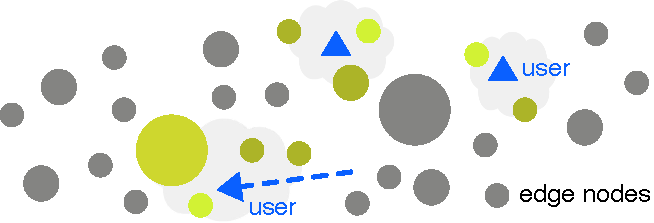
\includegraphics[width=0.9825\columnwidth]{morphing-concept.pdf}
    %%    \vspace{-2.0ex}
    \caption{Cloud morphing: the shape of a cloud dynamically follows the
      usage pattern}
    \Description{Clouds dynamically change their shapes.}
    \label{fig:concept}
  \end{center}
\end{figure}

\old{
  {\bf Cloud Morphing} is our vision for edge clouds in the future.
  By dynamically allocating microservices across distributed
  heterogeneous resources, a cloud service instance emerges at the best
  location and, as the usage pattern changes, the service instance also
  transforms the locations of the resources and their connections
  (Figure \ref{fig:concept}).
}

\new{
  {\bf Cloud Morphing} is our vision for future edge clouds, where a cloud service instance adapts to usage patterns, transforming the locations of the resources and their connections by dynamically allocating microservices across distributed and heterogeneous resources (Figure~\ref{fig:concept}).
  Microservice jobs are assigned to minimize the overall execution cost that includes computing, communication with the user, and database access. For instance, interactive tasks follow the user's location while data-intensive tasks remain close to the data, regardless of user location. Edge computing is formed automatically by allocating resources close to the users. Furthermore, services are inherently fault-tolerant and resilient against outages or disasters since faulty resources are automatically evicted from the resource pool.
}

\old{
  Microservice jobs are assigned so as to reduce the overall execution
  cost that includes computing, communication with the user, and access
  to database.
  For examples, an interactive task will follow the user when the user
  moves, while a data-intensive task will stay close to the data
  regardless of the user location.
  Edge computing is automatically formed by allocating resources close to
  the users.
  Moreover, services are inherently fault-tolerant and resilient
  against outages or disasters since faulty resources are
  automatically evicted from the resource pool.
}

%From the operational perspective, it can be viewed as virtualization
%of cloud infrastrcuture.
%Currently, cloud system operators manually manage physical servers and
%network switches to meet the overall demands.
%By decoupling physical resource management from service management,
%cloud service operators are liberated from hardware resource management.
%Moreover, it is not enough to shift responsibility to operators of the
%new lower infrastructure layer. We need a new self-managing
%infrastructure layer which does not require human operators.
\old{
  From the operational perspective, the physical resource management
  becomes simpler with a larger pool of small resources.
  Physical nodes can be easily attached to or detached from the resource pool.
  When there is a consistent hotspot, it can be alleviated or solved by
  placing new resources close to the hotspot and then attaching them to
  the resource pool at a convenient time.
}

\new{
  A larger pool of small resources simplifies physical resource management from an operational perspective. Physical nodes can be easily attached to or detached from the resource pool. When there is a consistent hotspot, new resources can be placed close to the hotspot and attached to the resource pool at a convenient time.
}

\old{
  Diverse resources would be owned and managed by different parties.
  It requires loose management of resources, as small parties cannot
  afford dedicated skilled operators.
  The utilization of each resource needs to be easily manipulated,
  without affecting the stability of the system.
  %% energy saving?
  Also, energy saving could be more critical for edge resources.
}

\new{
  Diverse resources would be owned and managed by different parties. This requires loose management of resources as small parties cannot afford dedicated skilled operators. The utilization of each resource must be easily manipulable without compromising system stability. Furthermore, energy savings could be crucial for edge resources.
}

\old{
  To realize such systems, it requires various technical advances across
  many fields.  Among other things, new autonomous resource management
  model is needed for distributed diverse resources,
  which is the topic of this paper.
}

\new{
  Realizing such systems requires technical advances across many fields. In particular, a new autonomous resource management model is needed for distributed diverse resources, which is the focus of this paper.
}

%%\subsection{Resource Management}

%% resource allocation problems are NP-hard
%% even harder for distributed heterogeneous resources
%Resource allocation in distributed clouds is a non-trivial
%optimization problem, and it is even harder when distributed
%management is assumed.
%% our idea: use congestion pricing mechanism for automatic load management
%To this end,
\old{
  We employ dynamic pricing for decentralized resource
  allocation which works as backpressure against congestion.
  By design, serious congestion never happens in the system as long as
  some resources remain available in the resource pool.
  It also reserves a sufficient margin essential for the performance of
  statistically multiplexing services.
  We use pseudo cost for manipulating resource allocation.
  Here, pseudo cost is not an actual monetary charge, but it is used to
  control resource utilization; it should not be confused with service
  fees for customers.
}

\new{
  We utilize dynamic pricing for decentralized resource allocation, which acts as backpressure against congestion. The system is designed to avoid serious congestion, provided that some resources remain available in the resource pool. This mechanism also reserves a sufficient margin essential for the performance of statistically multiplexing services. To manipulate resource allocation, we use pseudo cost, which should not be confused with service fees for customers. Pseudo cost is not an actual monetary charge; rather, it is used to control resource utilization.
}

\old{
  There exists a large body of literature formulating resource allocation
  as optimization problems.
  In this paper, we use terms and expressions borrowed from optimization
  theory. Our goal is, however, not to pursue theoretical optimum
  allocations, but to present a practical feedback control model for
  distributed resource management.
}

\new{
  Our paper draws on the extensive literature that formulates resource allocation as optimization problems. As such, we utilize terminology and expressions from optimization theory. However, our aim is not to pursue theoretical optimum allocations, but rather to present a practical feedback control model for decentralized resource management.
}

